% \documentclass[a4paper]{article}
% \usepackage{ctex}
\documentclass[AutoFakeBold]{ZafuThesis}

\academy{风景园林与建筑学院}%学院
\session{2024}%第*届
\author{买一盒、松手}%作者姓名
\studentNumber{20190000000000000}%学号
\myClass{建筑学191}%班级
\teacher{建筑系全体教师}{教授/副教授/讲师}%指导老师
\date{\today}%日期,显示在封面与诚信承诺书页
% \title{{浙江农林大学本科生毕业设计模板 }}%标题单行
\title{{浙江农林大学本科生}{毕业设计说明书或论文模板}}%标题双行
\entitle{Architectural design of Heshang Police Station of Xiaoshan District Public Security Bureau}%英文标题,显示在摘要页


\begin{document}
% %封面
\customCover

%自己的签名
\setsignature
  {
  
\includegraphics[width=100pt]{figures/MaiYihe}
  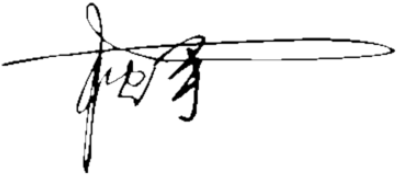
\includegraphics[width=120pt]{figures/SongShou}
  }
% 承诺页
\makestatement


%目录
\customContent

\frontmatter
%中文摘要,关键词分号分隔
\ZhAbstract
{
  摘要内容主要介绍所研究的课题内容、提出主要结论及创新之处。摘要部分格式:黑体加粗五号段前空两个汉字字符,摘要内容楷体五号,不超过300个汉字。关键词部分格式:黑体加粗五号段前空两个汉字字符,关键词内容楷体五号,术语用分号隔开,数量一般为3-6个。Abstract:Times New Roman加粗五号段前空两个汉字字符;Abstract内容:Times New Roman五号。Key Words: Times New Roman加粗五号段前空两个汉字字符; Key Words内容:Times New Roman五号,术语用逗号隔开。
  
}
{关键词1;关键词2;关键词3;关键词4;关键词5}


%英文摘要,关键词用逗号分隔
\EnAbstract
{In this short article we will discuss about LATEX for your dissertation}
{keyword 1, keyword 2, keyword 3}


\mainmatter
\section{使用说明}
ZafuTemplate(浙江农林大学本科生毕业设计说明/论文模板与开题报告模板)是厌倦了低效的Word的某人完成毕业任务时心血来潮所作,现发布到网上供浙江农林大学本科毕业生免费使用,在使用前请仔细阅读下面的内容和注意事项。\par
学校和学院的要求存在一定的差异,据了解,甚至同一学院的不同专业对论文模板的要求也有所不同(Zafu什么时候能统一一下啊!)。总之,本模版尚存不足之处,欢迎反馈,更希望大家能帮忙一起完善。
\subsection{目录下的文件说明}
\begin{itemize}
  \item ".vscode"是VSCode的配置文件(若使用别的编辑器可以忽略)
  \item "2024届毕设或论文材料要求"文件夹内包含学校要求说明与建筑学专业的示例文档
  \item "thesis"内是毕业设计说明/论文的LaTex模板{\bfseries 主体文件}
  \item "ZafuResearchProposal"内是开题报告的LaTex模板{\bfseries 主体文件}
\end{itemize}
\par
主题文件中'.tex' 文件是 LaTeX 文档的源文件。它包含实际的文档内容和 LaTeX 命令,用于生成最终的 PDF 文件;'.cls'文件是 LaTeX 文档类文件,定义了文档的整体布局和样式(如有需要,请在其中自行修改格式)。它包含了一组命令和宏,用于规范文档的格式;'figures'文件夹下为要在文中展现的图片;'.bib' 文件是用于存储参考文献的数据库文件。
\subsection{安装和配置}
请自行根据操作系统对映选择安装TeX发行版,在此不过多赘述。推荐使用VSCode编辑器编译运行。\par
教程推荐:\href{https://www.bilibili.com/video/BV12m4y1D7PZ/?vd_source=dfa6f0143619fda15de458493344dd04}{\textcolor{blue}{LaTeX论文写作指南——以VSCode编辑器为例}}\par
本模板主页:\href{https://github.com/Stolorzs/ZafuTemplatePublic}{\textcolor{blue}{ZafuTemplatePublic}}

\subsection{LaTex生成的PDF转化DOCX}
许多导师不会使用PDF编辑器从而要求学生提交DOCX批阅,或者学院要求提交DOCX格式的文档,迫于上述现实因素,不得不研究将LaTeX导出的PDF转化为DOCX格式的方法。\par
\paragraph{转化方式}
使用 Adobe Acrobat DC 打开 LaTeX 生成的 PDF 文件,然后选择“另存为 DOCX”即可完成转换。作者测试了 Adobe Acrobat DC 2023 及以上版本,绝大多数的字体格式与图片排版都能在Word中对映上,效果较好,但未对带公式的转化(因为咱建筑学写论文很少用公式)进行测试。
\paragraph{注意事项}
在 MacOS 下编译生成的PDF不要导出到Windows操作系统下转化,在 Windows 下编译生成的 PDF 也不要导出到 MacOS 操作系统下转化,不然字体的格式会发生错误。若转化效果欠佳,可以考虑将 PDF 拆分成多组内容,分组进行转化再合并。如,将毕业论文拆分为封面、诚信承诺书、目录、摘要、正文主体几部分内容,分组转化为DOCX后在Word中进行合并。

\subsection{免责声明}
本模板格式参照2024届毕设或论文材料要求内建筑学专业的示例文件所作。'.cls'格式的文件内容由本人原创,部分代码借鉴学习自兰州大学兰朵儿所作的本科毕业论文模板\href{https://github.com/yuhldr/LZUThesis2020}{
  ( \textcolor{blue}{点击可访问其GitHub页面})}。\par
作者的初衷是减少后人花费在格式调整上的无用功,使学弟学妹们能够专注于文章内容的写作,从而提高本科生的毕业论文/设计水平。作者不保证本模板完全符合学科要求,因使用本模板产生的损失{\bfseries 由使用者自负},作者{\bfseries 不承担任何责任}!

\section{文字格式}
\subsection{参考规范}
请使用者自行参阅毕业当年的《浙江农林大学本科生毕业论文(设计)系列材料》与学科给出的示例文件。
\subsection{排版规范}
\subsubsection{章节序号}
\subsubsection{文字颜色}
\subsubsection{字体加粗}
\subsubsection{引用方式}

\section{图片插入}
\section{表格绘制}
\subsection{excel2latex插件}
https://ctan.org/tex-archive/support/excel2latex/
\subsection{格式调整}

\section{代码框}

\section{数学公式}


% % 引用参考文献
% \clearpage
% \bibliographystyle{gbt7714-author-year}
% \bibliography{ref}

\Thanks
{
  岁月匆匆,大学时光如白驹过隙,我即将踏入毕业设计的最后阶段,心潮澎湃,回首往昔,感慨万千。在此,我要向所有曾经帮助、陪伴过我的人们深深地致以诚挚的谢意。\par
  首先,我要感谢母校,是她为我搭建了知识的殿堂,为我提供了探索未来的舞台。五年时光,荟萃了她对我的呵护与培育,我将永怀感恩之心。\par
  感谢建筑学院的恩师们,你们的悉心教导和引领,让我在学术之路上不断探索,不断超越。你们是我学习的灯塔,照亮了前行的道路。
}



\end{document}

